\documentclass[11pt]{beamer}
%
% Choose how your presentation looks.
%
% For more themes, color themes and font themes, see:
% http://deic.uab.es/~iblanes/beamer_gallery/index_by_theme.html
%
\mode<presentation>
{
  \usetheme{Darmstadt}      % or try Darmstadt, Madrid, Warsaw, ...
  \usecolortheme{default} % or try albatross, beaver, crane, ...
  \usefonttheme{default}  % or try serif, structurebold, ...
  \setbeamertemplate{navigation symbols}{}
  \setbeamertemplate{caption}[numbered]
} 
\usepackage[english]{babel}
\usepackage[utf8]{inputenc}
\usepackage{parskip}
\usepackage[T1]{fontenc}
\usepackage{lmodern,textcomp}  
\usepackage{hyperref}
\usepackage{amstext,amsmath}
\usepackage{dcolumn,booktabs}
\usepackage{amsfonts}
\usepackage{mathrsfs}
\usepackage{amssymb}
\usepackage{float}
\usepackage{listings}
\usepackage{url}
\usepackage{longtable}
\usepackage[tableposition=b]{caption}
\usepackage{color}
\usepackage{multicol}
\usepackage{verbatim}

\usepackage{subcaption}
\usepackage{pdflscape}
\usepackage{multirow}
\usepackage{array}
%\usepackage{appendixnumberbeamer}
\usepackage{graphicx}
\usepackage{booktabs}
\usepackage{comment}	



\title{Health for nothin' and the trade for free - \\ That ain't workin' ?! \\[0.5cm]
On the consequences of health on trade}
\author{Marius Grünewald}
\institute{Copenhagen University}
\date{17.06.2019}
\subject{Master Thesis Presentation}

\begin{document}

\begin{frame}[noframenumbering]
  \titlepage
\end{frame}

\begin{frame}{Outline}
  \tableofcontents
  \setcounter{framenumber}{1}
\end{frame}

\section{Motivation}

\begin{frame}{An interesting topic...}
\begin{figure}[!ht]
\begin{center}\caption{Exports and Health \label{Exports and Health}}
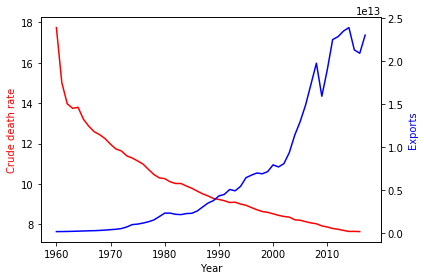
\includegraphics[width=0.6\textwidth]{C:/Users/mariu/Documents/Master_Thesis/Master_thesis/Pics_graphs/Trade_Health_World.png} \\
\smallskip {\footnotesize Figure \ref{Exports and Health} shows time trends of the crude death rate of the world (red)\\ and the aggregated world exports (blue).\\ The left scale measures the crude death rate per 1000, \\ while the right scale total exports in 2010 dollars. Both are measure are annual.}
\end{center}
\end{figure}
\end{frame}


\section{Theoretical Evidence}


\begin{frame}{The Environment}
The intermediate producers
\begin{align}
a_t + a_t^* = A_t N_t^{1-\alpha} K_{t-1}^{\alpha} \\
b_t^* + b_t = A_t^* N_t^{*^{ 1-\alpha}} K_{t-1}^{*^{\alpha}}
\end{align}
The final producers
\begin{align}
(\omega a_t^{\frac{\theta -1}{\theta}} + (1-\omega) b_t^{\frac{\theta -1}{\theta}})^{\frac{\theta}{\theta-1}} \\
((1-\omega) a_t^{*^{^\frac{\theta -1}{\theta}}} + \omega b_t^{*^{\frac{\theta -1}{\theta}}})^{\frac{\theta}{\theta-1}}
\end{align}
The resource constraints
\begin{align}
K_t - (1-\delta)K_{t-1} + C_t = (\omega a_t^{\frac{\theta-1}{\theta}} + (1-\omega) b_t^{\frac{\theta-1}{\theta}})^{\frac{\theta}{\theta-1}} \\
K_t^* - (1-\delta)K_{t-1}^* + C^*_t= ((1-\omega) a_t^{*^{\frac{\theta-1}{\theta}}} + \omega b_t^{*^{\frac{\theta-1}{\theta}}})^{\frac{\theta}{\theta-1}}
\end{align}
\end{frame}

\begin{frame}{Decentralized Solution}
Shocks occur to health
\begin{align}
H_{t} = \rho^H H_{t-1} + \epsilon_{t-1} \\ \text{which enters via}& \nonumber \\
\text{ln } A_{t} = \rho^A \text{ln } A_{t-1} + H_{t} \\
\text{ln } N_{t} = \rho^N \text{ln } N_{t-1} + H_{t}
\end{align}

Further note, the real exchange rate for the home country
\begin{align}
rer_t = \frac{qa_t}{qa_t^*}
\end{align}
and the home country's trade balance
\begin{align}
nx_t = q_{a,t} a_t^* - q_{b,t} b_t 
\end{align}


\end{frame}

\begin{frame}{Simulation}
\begin{figure}[!ht]
\begin{center} 
\begin{minipage}[t]{\textwidth}
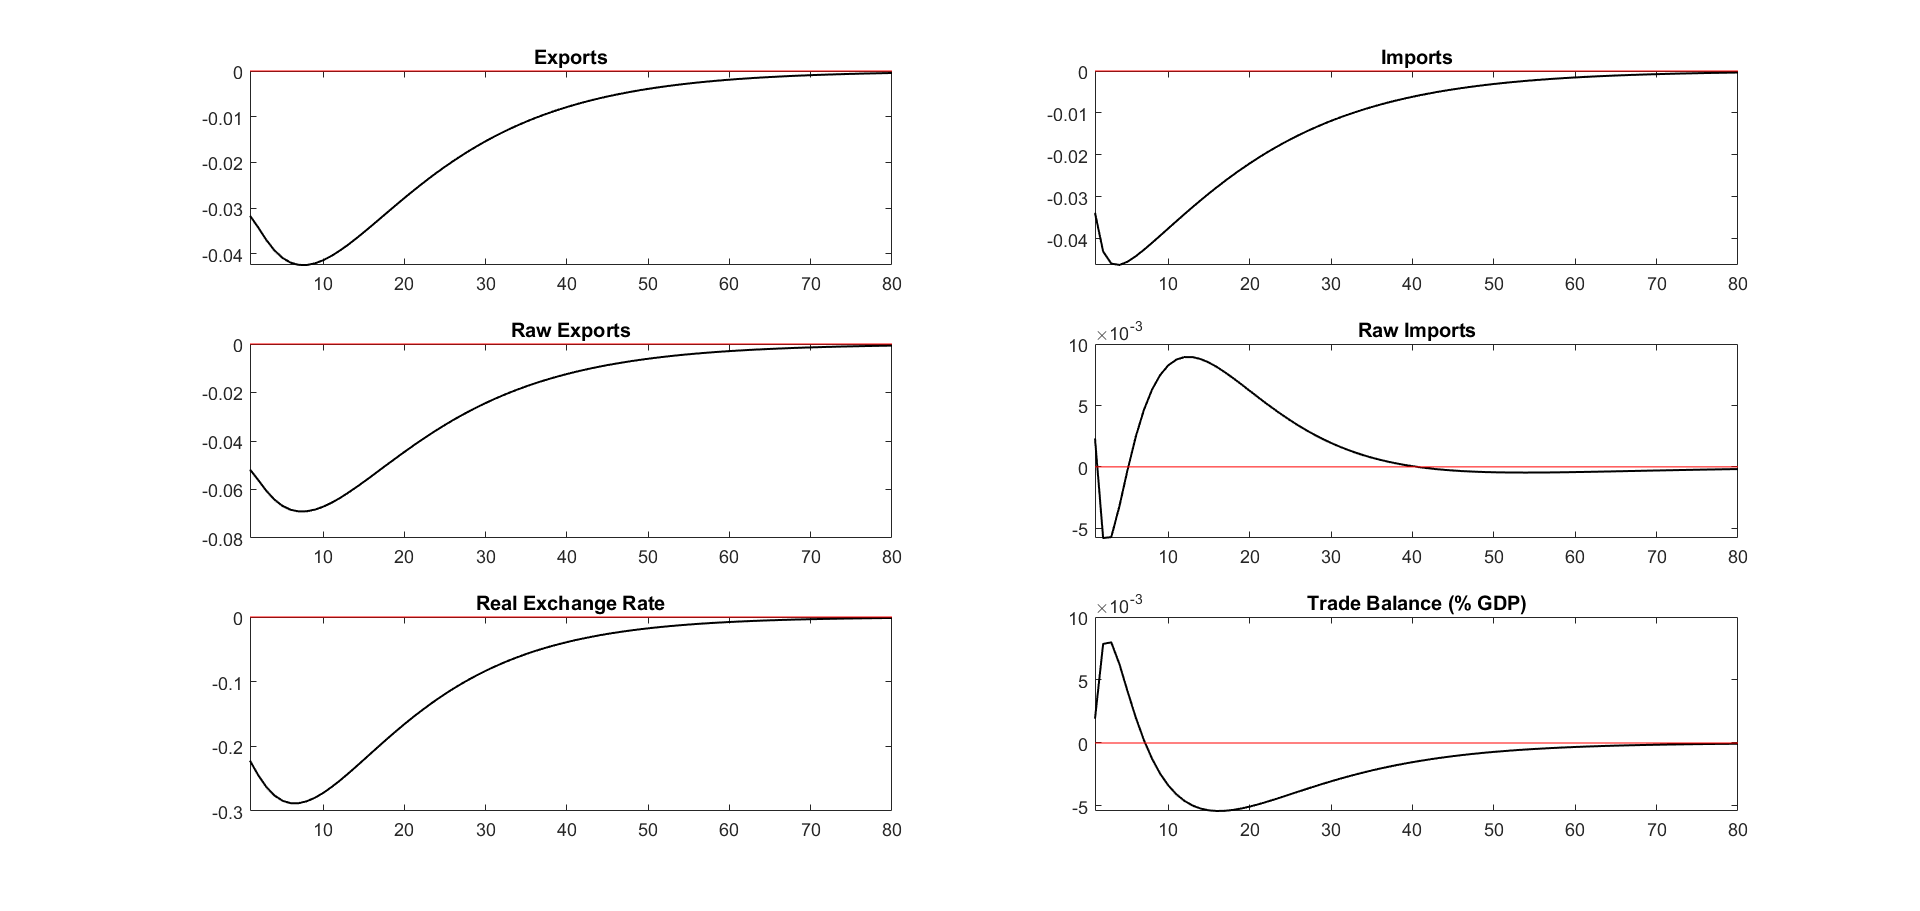
\includegraphics[width=1\textwidth]{C:/Users/mariu/Documents/Master_Thesis/Master_thesis/Pics_graphs/Simulation_expanded_1.png}\\
\caption{Simulation.\label{Simulation Evidence}}
\end{minipage}
\end{center}
\end{figure}
\end{frame}


\section{Data}

\begin{frame}{Measuring Ebola}

Overall sample properties 
\begin{itemize}
\item Covers 40 countries in Sub-Saharan Africa
\item For the years 2000 until 2016
\end{itemize}

I consider two main measures
\begin{itemize}
\item Case Prevalence Rate
\item Ebola Articles in NYT
\end{itemize}

\end{frame}


\begin{frame}{Other Data}
\begin{itemize}
\item Ebola Data from the \textit{WHO Situation reports}.

\item Health is measured in adult, age-adjusted mortality rates from the \textit{World Bank Development Indicators}.

\item Measures of trade include the logarithms of exports and imports as well as the trade balance (in \% of GDP). Data is taken from \textit{IMF Directions of Trade} dataset

\end{itemize}

\end{frame}


\section{Estimation Strategy}

\begin{frame}{Estimation Strategy}
In essence, my estimation strategy relies on a difference-in-differences to receive predicted mortality rates. \\
The (exogenous), predicted mortality rates work as an instrument for health to identify a causal mechanism of health on trade. \\
\begin{align}
Y_{ijt} =  \beta \mathbf{H_{it}} +  X_{ijt}'\eta + \alpha_{ij} + \zeta_t + \epsilon_{ijt}
\end{align}
with 
\begin{align}
\mathbf{H_{it}} =  \beta Z_{it} +  Q_{it}'\nu + X_{it}'\eta + \pi_{it} + \alpha_i + \zeta_t + \epsilon_{it}
\end{align}


\end{frame}

\section{Results}

\subsection{First Stage}

\begin{frame}
\begin{figure}[!ht]
\begin{center}
\begin{minipage}[t]{\textwidth}
\begin{minipage}[t]{0.5\linewidth}\caption{Pre-trends \label{Pre-trends}}
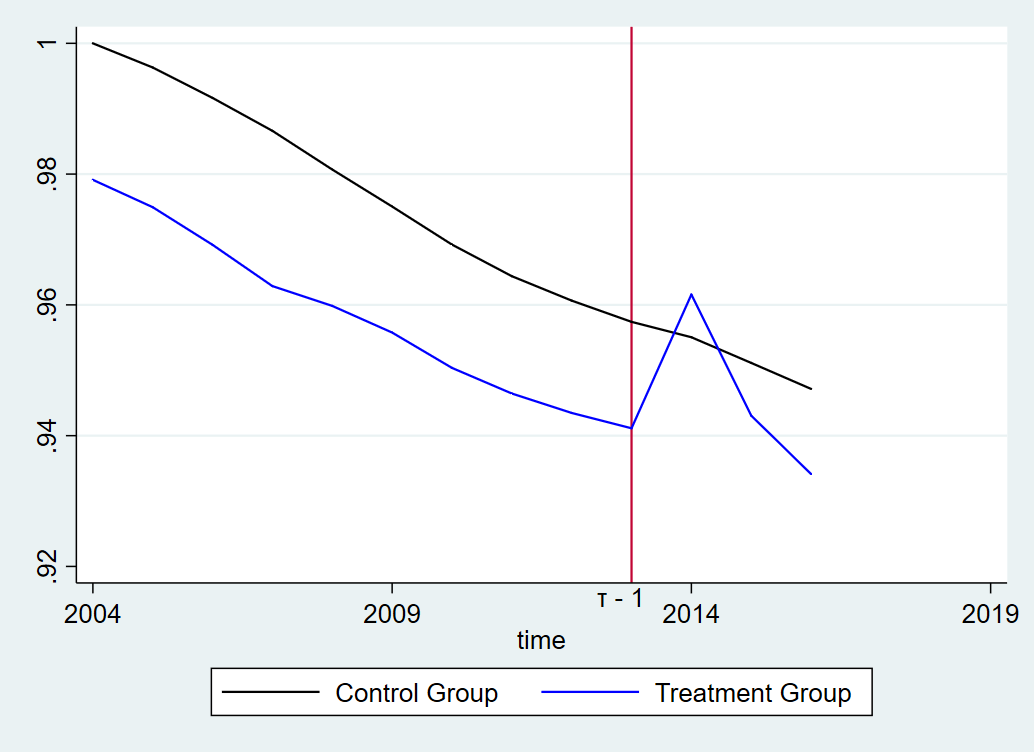
\includegraphics[width=\textwidth]{C:/Users/mariu/Documents/Master_Thesis/Master_thesis/Pics_graphs/Averages_pre_trends.png}\\
\end{minipage}\hfill% 
\begin{minipage}[t]{0.5\linewidth}\caption{Event Study \label{Event Study}}
\includegraphics[width = \textwidth]{C:/Users/mariu/Documents/Master_Thesis/Master_thesis/Pics_graphs/Event_study.png}\\
\end{minipage}\hfill% 
\end{minipage}
\end{center}
\end{figure}

\end{frame}


\begin{frame}{First Stage Results}

\begin{center}
\begin{table}[htbp]\centering  \caption{First stage results \label{First stage results}}
\resizebox{0.85\textwidth}{!}{
\begin{tabular}{lcc} \hline
Dependent Variable & \multicolumn{2}{c}{Log Adult Mortality Rate} \\ \hline
\vspace{4pt} & \begin{footnotesize}\end{footnotesize} & \begin{footnotesize}\end{footnotesize} \\
Log Prevalence Rate & 0.9716*** &  \\
\vspace{4pt} & \begin{footnotesize}(0.3169)\end{footnotesize} & \begin{footnotesize}\end{footnotesize} \\
Log Ebola Articles &  & 0.0203*** \\
 & \begin{footnotesize}\end{footnotesize} & \begin{footnotesize}(0.00389)\end{footnotesize} \\
\vspace{4pt} & \begin{footnotesize}\end{footnotesize} & \begin{footnotesize}\end{footnotesize} \\
Linear Trend & -0.0236*** & -0.0238*** \\
\vspace{4pt} & \begin{footnotesize}(0.00267)\end{footnotesize} & \begin{footnotesize}(0.00270)\end{footnotesize} \\
Observations & 124,117 & 124,117 \\
Number of country-pairs & 7,301 & 7,301 \\
Two-way FE & Yes & Yes \\
Cluster level & Country pair & Country pair \\
F-statistic & 39.60 & 69.58 \\ \hline
\multicolumn{3}{c}{\begin{footnotesize} \textit{Log Prevalence Rate} is the log of the number of infected divided by the total population \end{footnotesize} }\\
\multicolumn{3}{c}{\begin{footnotesize} \textit{Log Ebola Articles} is the log of the number NYT articles about Ebola and a country \end{footnotesize} }\\
\multicolumn{3}{c}{\begin{footnotesize} Clustered standard errors in parentheses. \end{footnotesize} }\\
\multicolumn{3}{c}{\begin{footnotesize} *** p$<$0.01, ** p$<$0.05, * p$<$0.1\end{footnotesize}} \\
\end{tabular}
}
\end{table}
\end{center}

\end{frame}


\begin{frame}{Clustered Standard Errors}
\begin{table}[htbp] \centering
\caption{Wild cluster bootstrap \label{Wild cluster bootstrap}}
\resizebox{\textwidth}{!}{
\begin{tabular}{lcccc} \hline
 & \multicolumn{2}{c}{(I)} & \multicolumn{2}{c}{(II)}  \\ \vspace{3pt}
Treatment group & \multicolumn{2}{c}{Three countries} & \multicolumn{2}{c}{Three countries}  \\ \vspace{3pt}
Treatment variable & \multicolumn{2}{c}{Case prevalence} & \multicolumn{2}{c}{Ebola articles} \\ \vspace{3pt}
Estimate & \multicolumn{2}{c}{0.9716} & \multicolumn{2}{c}{0.02} \\ \vspace{3pt}
Cluster robust s.e. & \multicolumn{2}{c}{0.3169} & \multicolumn{2}{c}{0.004} \\ \vspace{3pt}
t-statistic & \multicolumn{2}{c}{3.07} & \multicolumn{2}{c}{5.21} \\ \hline \vspace{3pt}
\vspace{3pt} P-values \& CI & P value & CI & P value & CI \\ \vspace{3pt}
Initial results & 0.004  & [0.331, 1.613] & 0.000  & [0.012, 0.028]\\ \vspace{3pt}
Bootstrap by country, restricted & 0.105 & [-631.6, 24.2] & 0.1054 &  [-.1698, .2974] \\ \vspace{3pt}
Bootstrap by country, unrestricted & 0.28& [-.461, 2.404] & 0.0000 & [.01224, .02828]  \\ \vspace{3pt}
Bootstrap by country-pair, restricted & 0.0856 & [-1.649, 5.502] & 0.009 & [.009949, .03193] \\ \vspace{3pt}
Bootstrap by country-pair, unrestricted & 0.1381 & [-.5862, 2.529] & 0.000 & [0.012, 0.028] \\ \hline \vspace{3pt}
\end{tabular}
}
\end{table}
\end{frame}

\subsection{Second Stage}


\begin{frame}{Baseline Results}
\begin{table}[htbp] \centering
\caption{Second Stage Baseline \label{Second Stage Baseline}}
\resizebox{\textwidth}{!}{
\begin{tabular}{lcccccc} \hline
 & (1) & (2) & (3) & (4) & (5) & (6) \\
Dependent Variable & \multicolumn{2}{c}{Exports} & \multicolumn{2}{c}{Imports}  & \multicolumn{2}{c}{Trade Balance (\% GDP)}  \\ \hline
\vspace{4pt} & \begin{footnotesize}\end{footnotesize} & \begin{footnotesize}\end{footnotesize} & \begin{footnotesize}\end{footnotesize} & \begin{footnotesize}\end{footnotesize} & \begin{footnotesize}\end{footnotesize} & \begin{footnotesize}\end{footnotesize} \\
Log Mortality Rate & -3.1353*** & -3.179*** & 0.0591 & 0.0649 & 0.0172 & 0.0173\\
 & \begin{footnotesize}(0.673)\end{footnotesize} & \begin{footnotesize}(0.675)\end{footnotesize} & \begin{footnotesize}(0.0499)\end{footnotesize} & \begin{footnotesize}(0.0494)\end{footnotesize} & \begin{footnotesize}(0.0134)\end{footnotesize} & \begin{footnotesize}(0.0141)\end{footnotesize} \\
\vspace{4pt} & \begin{footnotesize}\end{footnotesize} & \begin{footnotesize}\end{footnotesize} & \begin{footnotesize}\end{footnotesize} & \begin{footnotesize}\end{footnotesize} & \begin{footnotesize}\end{footnotesize} & \begin{footnotesize}\end{footnotesize} \\
Log GDP p.c. &  &  & &  & 0.0067 & 0.0067 \\
 & \begin{footnotesize} \end{footnotesize} & \begin{footnotesize} \end{footnotesize} & \begin{footnotesize} \end{footnotesize} & \begin{footnotesize} \end{footnotesize} & \begin{footnotesize}(0.0091)\end{footnotesize} & \begin{footnotesize}(0.0092)\end{footnotesize} \\
\vspace{4pt} & \begin{footnotesize}\end{footnotesize} & \begin{footnotesize}\end{footnotesize} & \begin{footnotesize}\end{footnotesize} & \begin{footnotesize}\end{footnotesize} & \begin{footnotesize}\end{footnotesize} & \begin{footnotesize}\end{footnotesize} \\
Instrument & Prevalence & Articles & Prevalence & Articles & Prevalence & Articles \\
\vspace{4pt} & \begin{footnotesize}\end{footnotesize} & \begin{footnotesize}\end{footnotesize} & \begin{footnotesize}\end{footnotesize} & \begin{footnotesize}\end{footnotesize} & \begin{footnotesize}\end{footnotesize} & \begin{footnotesize}\end{footnotesize} \\
Observations & 57,794 & 57,794 & 64,203 & 64,203 & 81,872 & 81,872 \\
Two-way FE & Yes & Yes & Yes & Yes & Yes & Yes \\
F-statistic first stage & 34.53 & 47.49 & 41.77 & 58.36 & 27.95 & 35.64 \\
No. of clusters & 40 & 40 & 40 & 40 & 38 & 38 \\
Cluster & &\multicolumn{2}{c}{Country pair} \\ \hline
\multicolumn{7}{c}{\begin{footnotesize} Clustered standard errors in parentheses. \end{footnotesize} }\\
\multicolumn{7}{c}{\begin{footnotesize} *** p$<$0.01, ** p$<$0.05, * p$<$0.1\end{footnotesize}} \\\end{tabular}
}
\end{table}
\end{frame}

\begin{frame}{Impulse Response Functions}
\begin{figure}[!ht]
\begin{center}
\begin{minipage}[t]{\textwidth}
\begin{minipage}[t]{0.3\linewidth}\vspace{0pt} 
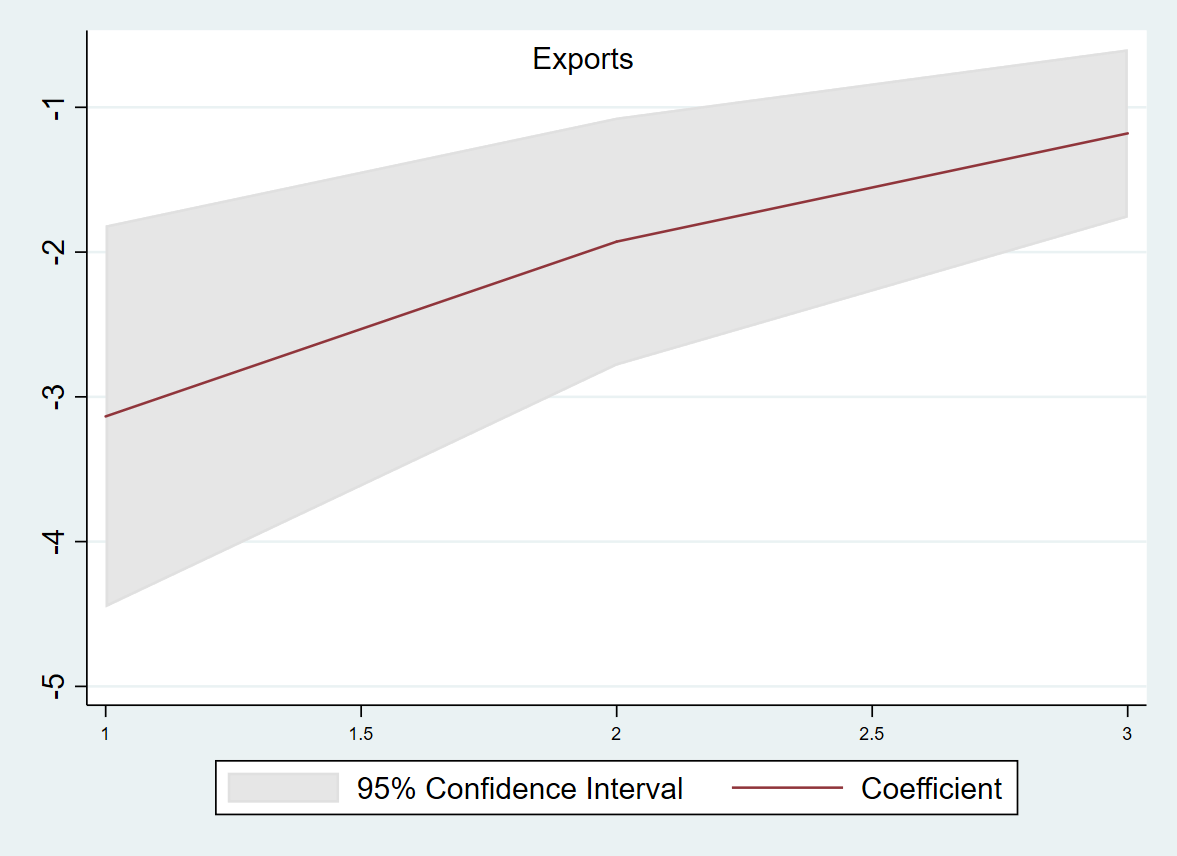
\includegraphics[width=40 mm]{C:/Users/mariu/Documents/Master_Thesis/Master_thesis/Pics_graphs/IRF_second_exp_prev.png}\\
\end{minipage}\hfill% 
\begin{minipage}[t]{0.3\linewidth}\vspace{0pt} 
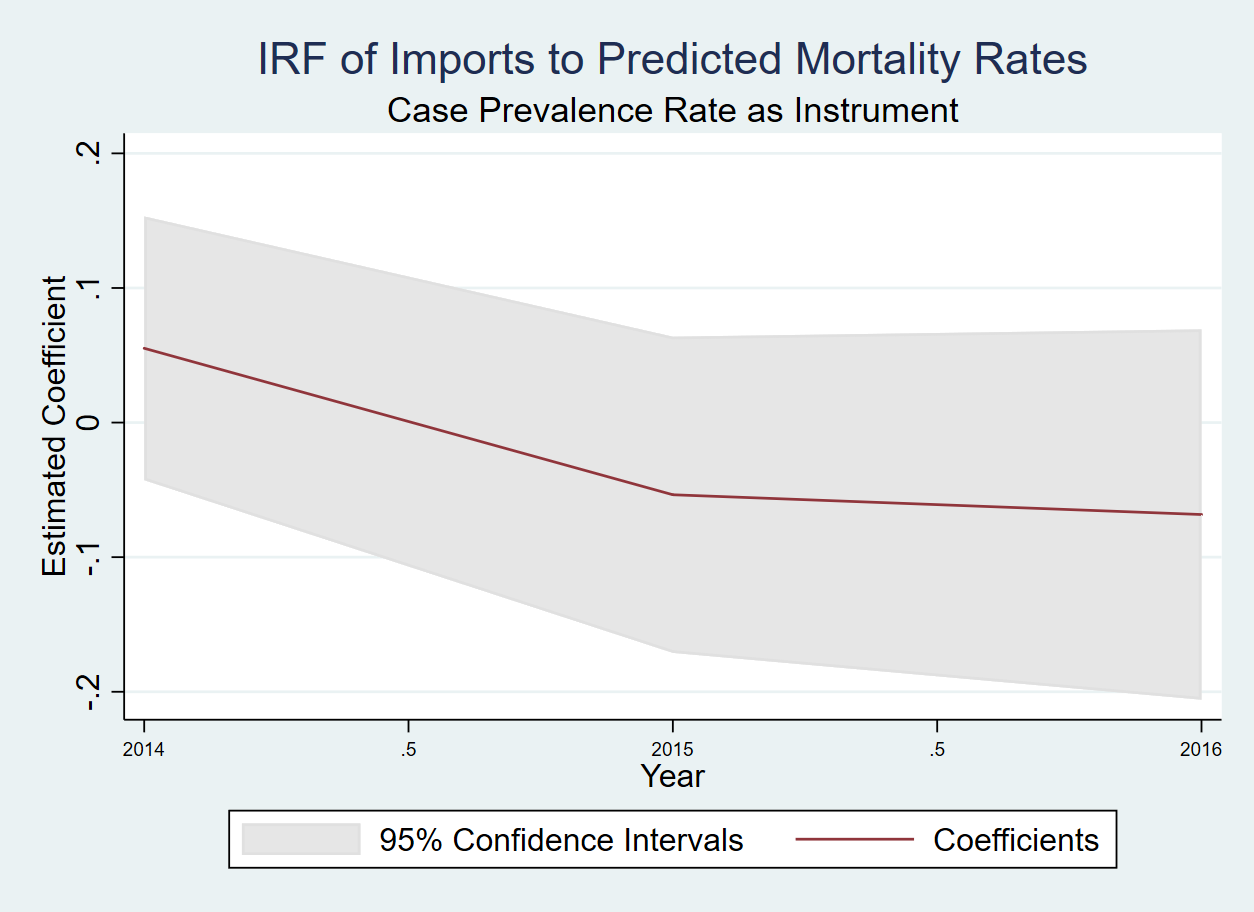
\includegraphics[width=40 mm]{C:/Users/mariu/Documents/Master_Thesis/Master_thesis/Pics_graphs/IRF_second_imp_prev.png}\\
\end{minipage}\hfill% 
\begin{minipage}[t]{0.3\linewidth}\vspace{0pt} 
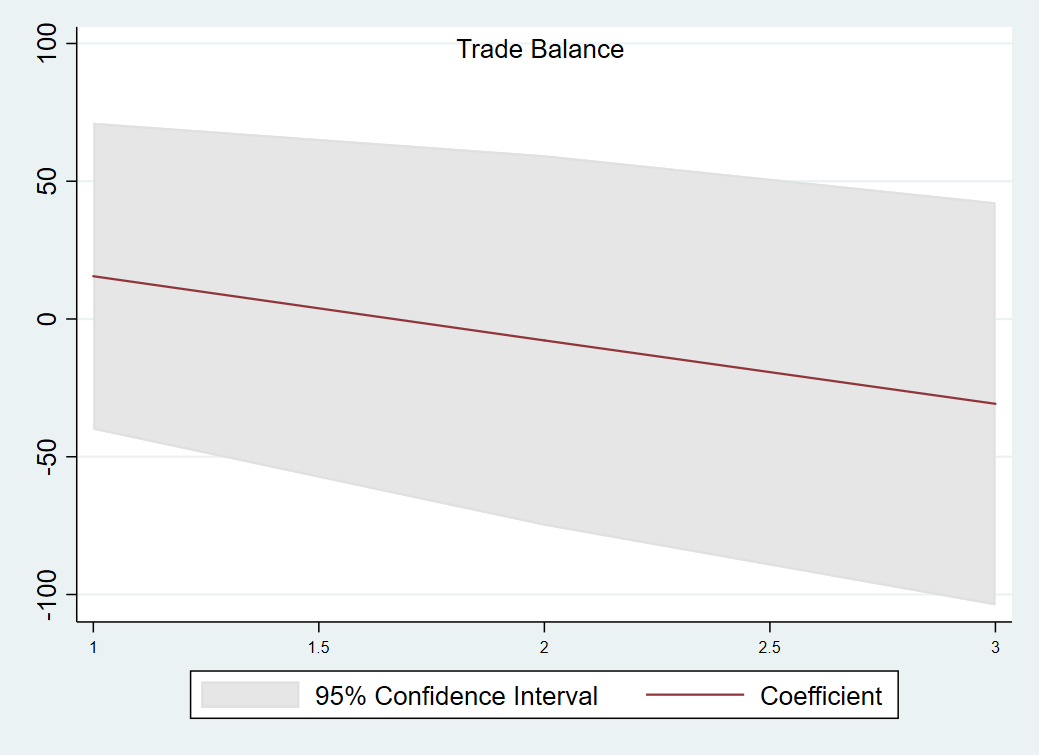
\includegraphics[width=40mm]{C:/Users/mariu/Documents/Master_Thesis/Master_thesis/Pics_graphs/IRF_second_tb_prev.png}\\
\end{minipage}\hfill%
\caption{Second Stage IRF\label{Second Stage IRF}}
\end{minipage}
\end{center}
\end{figure}
\end{frame}

\section{Conclusion}
\begin{frame}{Let's wrap it up}
\begin{itemize}
\item An increase in the Ebola prevalence rate by 1 \% cause mortality rates to climb by 1\% to 1.5\%.  \\
\item Increase in mortality rates by 1\% can be associated with a reduction of exports by between 2\% and 3 \%. \\
\item Likely no impact on imports or trade balance. \\
\item Micro-approach to investigate the exact mechanism \\
\item Longer time horizon. \\
\item To policy-makers: Effective spending on health to increase exports, potentially, threefold.
\end{itemize}
\end{frame}


\end{document}